
%% [STABILITY]
%%________________________________________________________
\section{Stability of the beam pattern}


\subsection{Individual scan beam profiles}

We checked the stability of the beam against various observing
condition (source intensity, weather condition, focus optimisation) by
comparing the beam profile of the beam-map set, which comprizes nine
beam-maps acquired from N2R8 to N2R10, as defined in
Sect.~\ref{se:beammap_set}.
The nine beam profiles and their ratio
w.r.t. the median beam profile are shown in Fig.~\ref{fig:beam_prof}.


\begin{figure}[h]
  \centering
  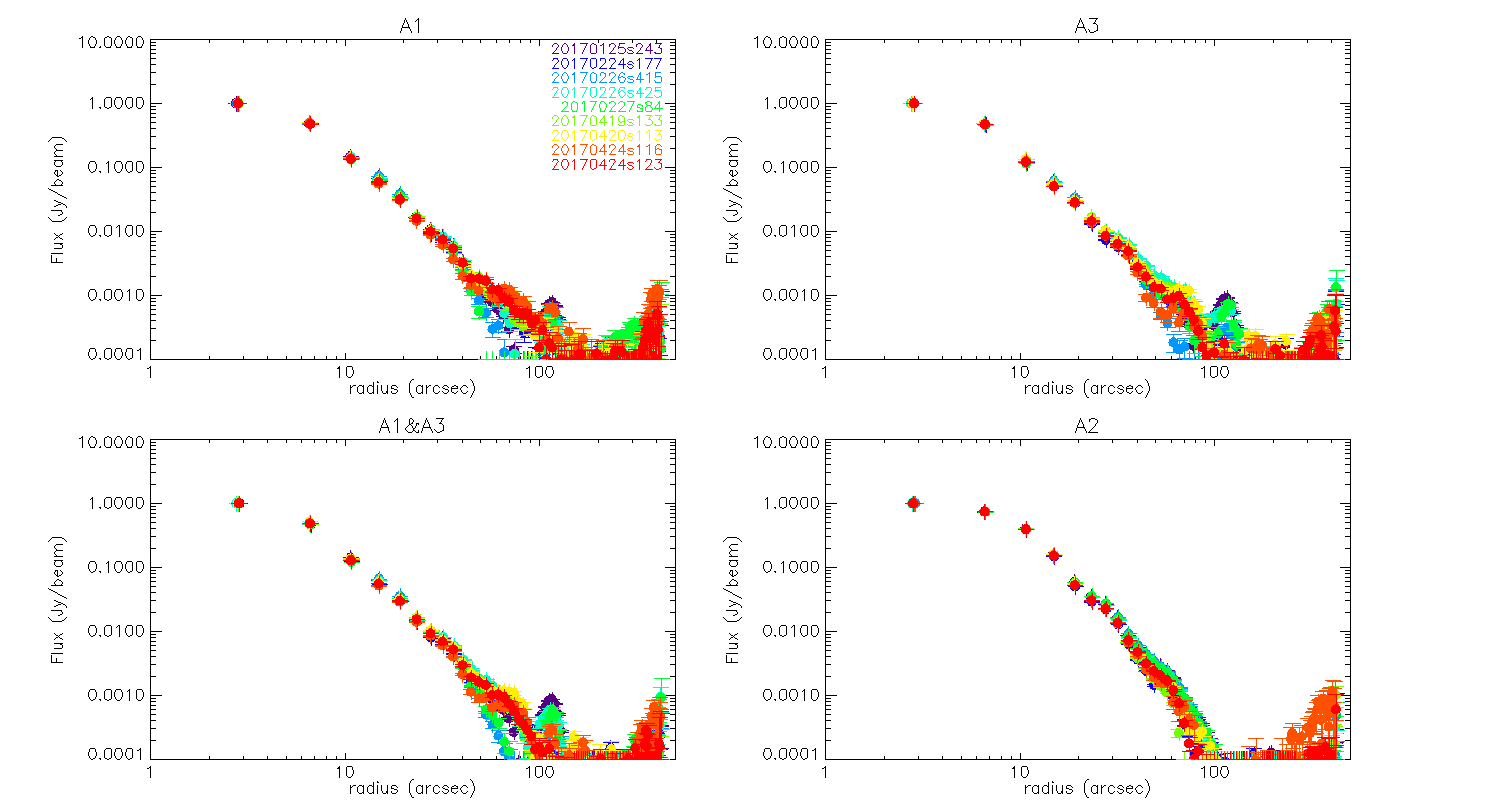
\includegraphics[clip=true,width=\textwidth]{Figures/Profile_allscans_mixed}
  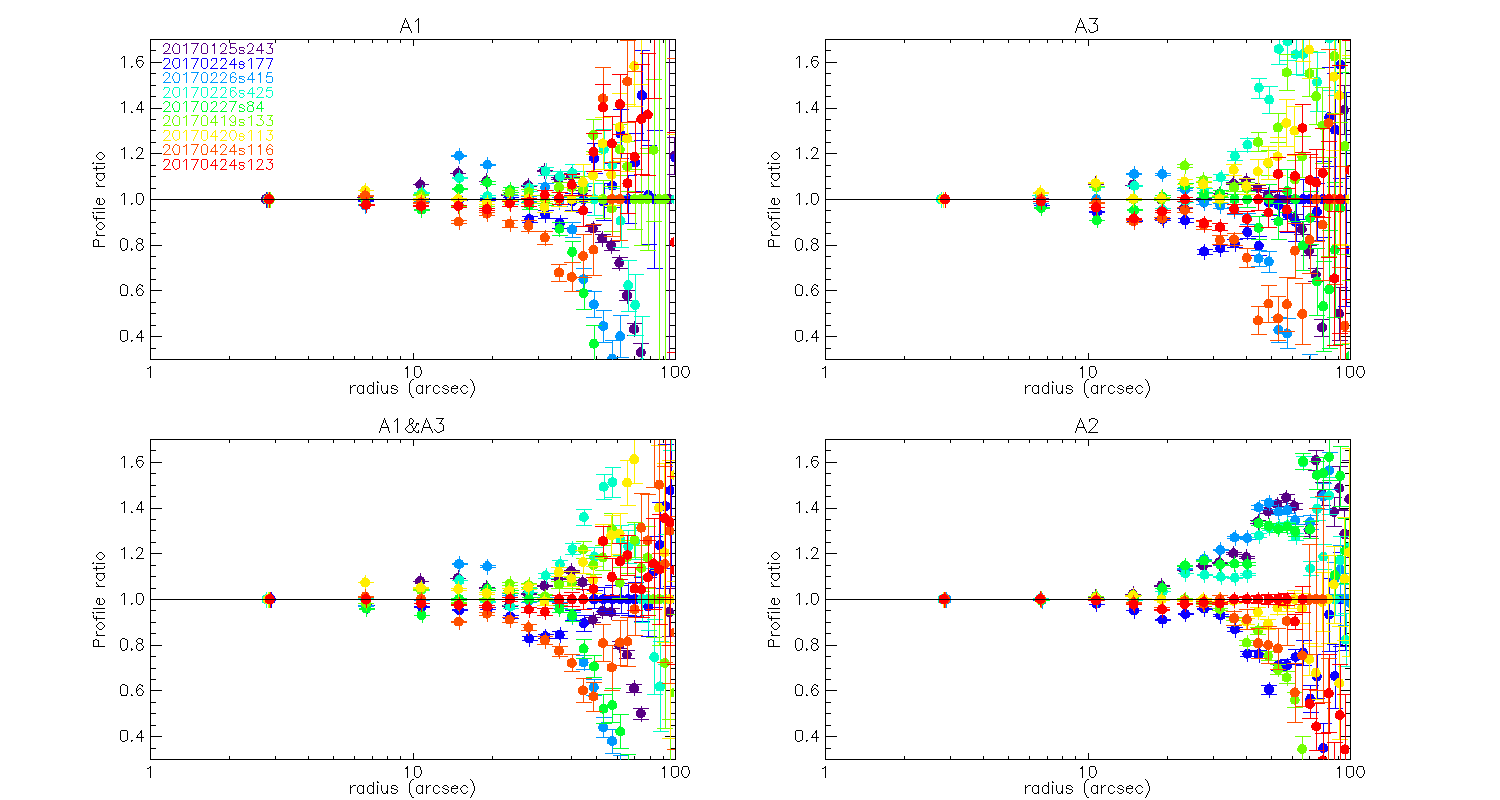
\includegraphics[clip=true,width=\textwidth]{Figures/Profile_allscans_over_median_mixed}
\caption[Stability of the beam profile]{Beam profiles from various N2R8 to N2R10
  beam-map scans. The upper panel shows the beam profiles normalised
  to the maximum value, and the lower panel the ratios w.r.t. the median profile.}
  \label{fig:beam_prof}
\end{figure}


\subsection{Main beam FWHM stability}

[A FAIRE:

  AJOUTER LES PLOTS DE STABILITE EN FONCTION DE ELEVATION, TAU

]
